\section[Theorie]{Theorie \textnormal{\cite{germanium}}}
\label{sec:theorie}

Zum Verständnis des hochreinen Germaniumdektektors werden die theorethschen Grundlagen dessen im Folgenden erläutert.

\subsection{Die Wechselwirkung von Strahlung mit Materie}
\label{sec:WW mit Materie}

Bei der Gamma-Strahlungs-Detektion werden Elektronen des Detektor-Matrials von den Gamma-Photonen angeregt und damit werden die 
Atome ionisiert. Daher bilden sich Elektronen-Loch-Paare. Die Primärenelektronen ionisieren wiederum weitere Atome des Detektor-Mediums und erzeugen somit weitere Elektron Loch Paare.
Die Anzahl der Elektronen-Loch Paare ist direkt proportional zur Energie des Elektrons aus der primären
Wechselwirkung.

Da der Absorbtionskoeffizient für Gamma-Strahlung bei Gasen sehr niedrig ist, 
werden Gamma-Strahlen-Detektoren aus Festkörpern gebaut. Das Matrial des Detektors muss so gewählt werden, dass
die Anzahl Elektronen-Loch-Paare gesammelt und als elektrisches Signal wiedergegeben werden kann.
Zusätzlich ist der Grad der Interaktion von Gamma-Strahlung mit Materie abhängig von der Energie der Strahlung.
Der Intensitätsverlust  eine $\gamma$-Strahls in Materie ist abhängig von der jeweiligen Schichtdicke des Materials $d$,
der Elektronendichte und dem Wirkungsquerschnitt $\sigma$. Dabei ist der Wirkungsquerschnitt ein Maß für die Wahrscheinlichkeit einer Teilchenreaktion.
Dieser lässt sich als effektive Wirkungsfläche interpretieren

In Abbildung \ref{fig:koeffizient} ist der Dämpfungskoeffizient von Germanium, welcher die Reduktion der Strahlungsintensität
bei bestimmter Energie verursacht durch den Absorber misst, gegen die Gamma-Strahlen Energie aufgetragen.


\begin{figure}[H]
    \centering
    \includegraphics[width=0.5\textwidth]{content/grafik/dämpfungskoeffizientGermanium.jpg}
    \caption{ \cite{gamma_ray}}
    \label{fig:koeffizient}
\end{figure}

Die totale Kurve setzt sich aus verschiedenen Komponenten zusammen: Der Photoeffekt, der Compton Effekt und die Paarerzeugung.
Im Folgenden werden die einzelnen Komponenten erläutert.

\subsubsection{Der Photoeffekt}
\label{sec:photoeffekt}

Der Photoeffekt beschreibt den Prozess bei dem ein ein Gamma-Quant mit einem Hüllenelektron wechselwirkt.
Das Photon wird absorbiert, daher gibt es seine gesamte Energie an das Atom ab, und ein Elektron wird emittiert. 
Das Atom nimmt dabei den Rückstoßimpuls auf und wird ionisiert.
Anhand der Abbildung \ref{fig:koeffizient} lässt sich ablesen, dass für Energie im Bereich bis zu \qty{100}{\kilo\eV} 
Absorbtion durch den Photoeffekt dominiert. Der Wirkungsquerschnitt des Photoeffekts fällt für große Energien ab.
Bei konstanter Photonen-Energie nimmt $\sigma$ stark zu für wachsende $Z$.
Demnach ist der Wirkungsquerschnitt abhängig von Energie der der $\gamma$-Quanten und der Kernladungszahl $Z$.
%Für natürliche Strahler ergibt sich $ \sigma_{\text{Ph}} \sim Z^{\alpha} / E^{\delta} $

\subsubsection{Der Compton Effekt}
\label{sec:compton}

Der Compton-Effekt ist die Streuunug eines Photons an einem quasi-freien oder freien Elektron.
Die Hüllenelektronen eines Atoms werden hier als quasi-frei betrachtet unter der Bedingung, dass
die Enrgie des Photons viel größer als die Bindungsenergie der Elektronen ist. Dieser Prozess
dominiert in Materie um \qty{1}{\mega\eV}.
Die Kinematik der Compton Streuung ist in Abilldung \ref{fig:compton} zu sehen.

\begin{figure}[H]
    \centering
    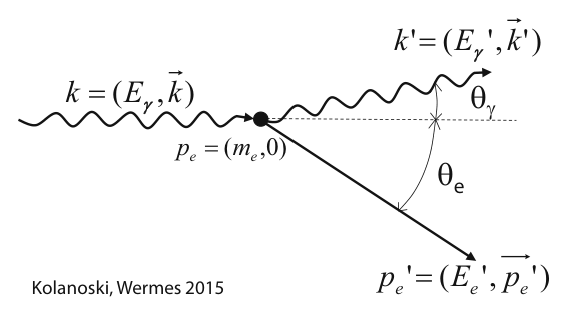
\includegraphics[width=0.5\textwidth]{content/grafik/compton.jpg}
    \caption{Die Kinematik des Compton Effekts, wobei das Elektron als quasi-frei betrachtet wird.\cite{teilchendetektoren}}
    \label{fig:compton}
\end{figure}

Um den Zusammenhang zwischen der Energie und des Winkels des gestreuten Photons
zu brechenen, werden Viererimpulse verwendet. Diese wurden in der Abbildung \ref{fig:compton} definiert.
Dabei bezeichnen $k$ und $p_{\text{e}}$ die Viererimpule des Photons und des Elektrons vor dem Stoß.
$k'$ und $p_{\text{e}}'$ bezeichen die Viererimpulse nach dem Stoß.
Aus Impulerhaltung und Energieerhaltung folgt der Zusammenhang
\begin{equation}
    E_\gamma^{\prime}=\frac{E_\gamma}{1+\epsilon\left(1-\cos \theta_\gamma\right)}
    \label{eqn:Energie_comptonstreuung}
\end{equation}
für die Energie des gestreuten Photons.

Den Wirkungsquerschnitt der Compton Streuung ergibt sich aus der Integration der Klein-Nishina-Formel über den Raumwinkel
\begin{equation}
    \frac{d \sigma}{d \Omega}=\frac{r_e^2}{2\left[1+\epsilon\left(1-\cos \theta_\gamma\right)\right]^2}\left(1+\cos ^2 \theta_\gamma+\frac{\epsilon^2\left(1-\cos \theta_\gamma\right)^2}{1+\epsilon\left(1-\cos \theta_\gamma\right)}\right).
\end{equation}
Für den differentiellen Wirkungsquerschnitt in Abhängigkeit zur Energie ergibt sich 
\begin{equation}
    \frac{d \sigma}{d E} = \frac{\pi r_{\text{e}}}{\epsilon E_\gamma} \left(2 - \frac{2 E}{\epsilon \left(E_\gamma - E \right)}+ \frac{E^2}{\epsilon^2 \left(E_\gamma - E \right)^2} + \frac{E^2}{E_\gamma \left(E_\gamma - E \right)}\right).
\end{equation}

Für den Wirkungsquerschnit pro Atom kommt es zu einer linearen Abhängigkeit
\begin{equation}
    \sigma_{\text{Compton}}^{\text{Atom}}=Z \sigma_{\text{Compton}}.
\end{equation}

Die Linearität gilt für die Annahme von freien Elektronen, also für Energien oberhalb der
Bindungsenergie des Elektronen.
Für kleinere Energien der Compton Wirkungsquerschnitt in Materie ab.

\subsubsection{Die Paarerzeugung}
\label{paarerzeugung}

Eine weitere Wechselwirkung ist die Paarerzeugung, wobei ein Photon mit dem ganzen Atom interargiert.
Das $\gamma$-Quant kann in dem Coulomb Feld einer Ladung in ein Elektron-Positron-Paar umgewandelt werden.
Aufgrund der Impulserhaltung kann Paarerzeugung nur auftreten, wenn ein Stoßpartner in Form eines Atoms oder eines Hüllenelektrons
gegeben ist.
Damit Paarbildung auftreten kann, muss für Energie der Photonen die Bedingung 
\begin{equation}
    E_\gamma \approx 2 m_e c^2
\end{equation}
erfüllt sein. 
Zusammen mit der Abbildung \ref{fig:koeffizient} folgt, dass die Paarerzeugung für Energien größer als \qty{1}{\mega\eV} dominiert.

\subsection{Grundlagen eines Halbleiter-Detektors}
\label{sec:Halbleiter-Detektor}

Halbleiterdetektoren aus Silizium oder Germanium eigenen sich für den Nachweis von Gammastrahlung und die Bestimmung derer Energie mit einer hohen Gnauigkeit.
Die zentrale Komponente des Detektors ist die Halbleiterdiode. In diesem Versuch wird ein Germaiumdektektor verwendet.
Die Diode besteht aus einem zylinderförmigen Germanium Kristall. Die Oberfläche ist über Eindiffusion von Lithium Atomen n-dotiert.
An diese wird der Pluspol der Sperrspannung angelegt. Im Inneren des Kristalls befindet sich eine koaxiale Bohrung, welche an der Oberfläche mit Gold bedampft wurde, sodass diese p-dotiert ist.
Es kommt zur Ausbildung einer ausgedehnten Verarmungszone. Wenn nun die Gammastrahlung ,bei einer Energie $E_{\gamma} $ oberhalb der Bandlücke, eintrifft, wird ein Primärelektron von dem Photon angregt.
Sodass das Elektron von dem Valenzband in das Leitungsband angehoben wird. Wird eine Elektron in ein anderes höher liegendes Band angregt, lässt dieses eine freie Stelle über. 
Diese wird als Loch mit einer positiven Ladung interpertiert.
Die Energie dieses Elektrons ist sehr hoch, daher kommt es mehrfach zu Anregung von Sekundärteilchen, welche wiederum freie Stellen zurücklässt. Die Erzeugung von sekundäre Elektronen ist ein statistischer Prozess.
Da die Löcher als Teilchen mit positiver Ladung angesehen werden können und die Elektronen eine negative Ladung besitzen, werden die Löcher von der n-dotierten Schicht und die Elektronen von der p-dotierten Schicht angezogen.
So fließt ein Strom der gemessen werden kann.
Die Anzahl der Elektronen-Loch-Paare $n$ ist direkt abhängig zu der absorbierten Energie der Gammastrahlung $E_{\text{absorbiert}}$. Für die Energie $\epsilon$, die benötigt wird,
um ein Elektron-Loch-Paar zu erzeugen gilt der Zusammenhang

\begin{equation}
    n = \frac{E_{\text{absorbiert}}}{\epsilon}.
\end{equation}

Die Elektronen und die Löcher müssen in dem Detektormatreial gut mobil sein. Die größe des Kristalls ist ebenfalls eine nicht zu vernachlässigende Eigenschaft.
Wichtig ist dass der Absobtionskoeffizient groß ist, damit die Messung effektiv ist. Um dies zu garantieren werden Materialien mit einem großen Absobtionskoeffizient
gewählt. Dieser hängt mit der Kernladungszahl $Z$ zusammen. Das Matrial muss zudem elektrische Charakteristika aufweise, da ein Stromimpuls gemessen werden soll. Zusammen mit der Mobiltät, die für die
Elektronen und die Löcher gelten soll, kann der Schluss gezogen werden, dass sich Halbleiter gut für solche Detektoren eignen.

In der Abbildung \ref{fig:halbleitermatrialien} sind einige Materialien,welche sich eignen würden für einen Halbleiterdetektoren und deren Eigenschaften.

\begin{figure}[H]
    \centering
    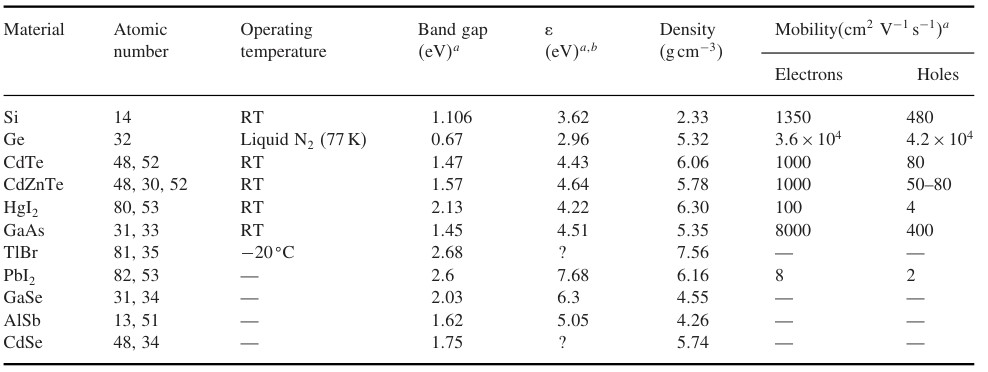
\includegraphics[width=0.8\textwidth]{content/grafik/passende.jpg}
    \caption{Die Eigenschaften einiger Materialien, welche geeignet wären zur Detektion von Gammastrahlung.\cite{gamma_ray}}
    \label{fig:halbleitermatrialien}
\end{figure}

\subsection{Das Spektrum eines monochromatischen Gammastrahlers}
\label{sec:Gammastrahlung}

Das Gammaspektrum weist verschiedene charakteristische Stellen auf. In Abbildung \ref{fig:gamma-cs} ist das Gammaspektrum von
Cs-137 beispielhaft gezeigt.

\begin{figure}[H]
    \centering
    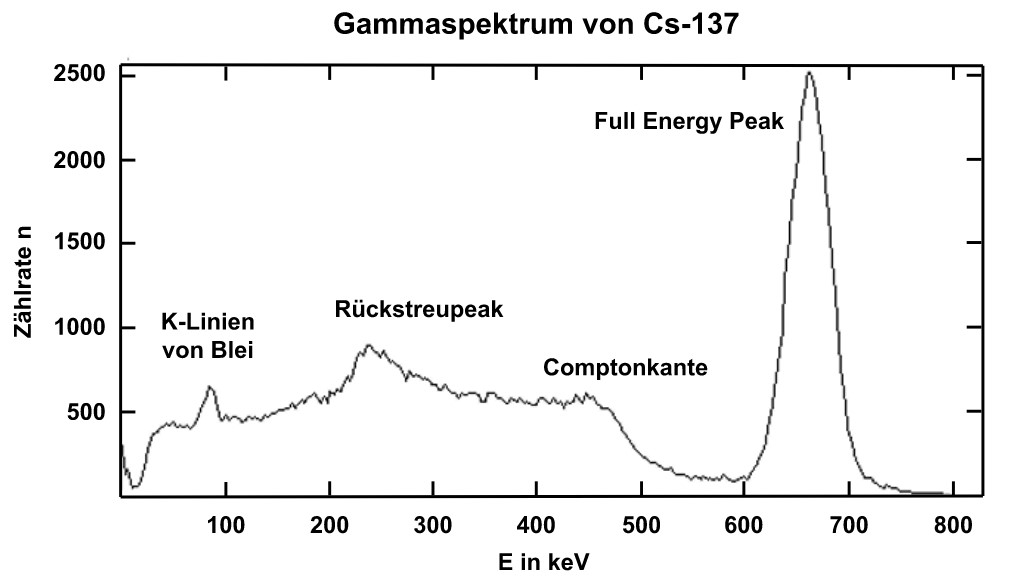
\includegraphics[width=0.8\textwidth]{content/grafik/Gammaspektrum.jpg}
    \caption{Das Gammaspektrum von Cs-137. \cite{Gammaspektrum}}
    \label{fig:gamma-cs}
\end{figure}

Existenziell für die Bestimmung der Gammenergien ist der Photopeak oder auch der Full Energy Peak.
Er gibt die gesamte Energie des einfallenden $\gamma$-Quants an. Nur wenn der Photoeffekt stattgefunden hat ist die Deponierung der #
gesamten Energie im Detektor möglich.